\chapter*{Conclusions and perspectives} 
\addcontentsline{toc}{chapter}{Conclusions and perspectives} % aggiunge la bibliografia all'indice
 
Several simulations of the \textit{apo} and \textit{holo} forms of the MBP  in powder environment were performed. 
A lot of the data and, in particular, the final configurations of the simulated systems were stored. The first analysis of the trajectory were carried out and some of the results were reported in chapter three. In particular, interesting small differences on the MSD calculated at low temperature -- 200 K and 220 K -- for the MBP and the MBP+Malt powder systems were found; and significant variations of the MSD amplitude were observed changing the model of the forcefield for the water molecules. 

Therefore, the thesis, with its results, provided a crucial base for the study of entropic contributions to the formation of the MBP+Malt complex. 

The coordinates and the velocities reported from the simulations can be used to rapidly perform others simulations of the studied systems in different conditions -- for instance, changing the temperature or the sampling frequency.

The simulations were carried out to enable subsequent studies combined with neutron scattering data.

In particular, the simulation of 1 $\mu s$ of the MBP and MBP+Malt systems, will allow to perform, for the first time, a clustering analysis on powder systems to investigate the changes upon the configurational entropy upon the complexation. 

\appendix
\chapter{Graphs resulting from the MSD calculations}\label{apendix:MSD}
\noindent
In the following pages some of the graphs are displayed, resulting from the calculation of the MSD performed from the simulated trajectories.\\
\\
Page 66 -- \textbf{MSD of the powders as a function of the temperature}:
\textit{the value of $t_w$ were chosen to correspond approximately to the sensibility of neutron scattering experiments}\\
\\
Page 67 -- \textbf{MSD of the H$_2$O of the powders as a function of the temperature}:
\textit{the value of $t_w$ were chosen to correspond approximately to the sensibility of neutron scattering experiments}\\
\\
Page 68 -- \textbf{MSD as a function of the time window at 220 K}:
\textit{some interesting differences between the MBP and the MBP+Malt systems are shown}\\
\\
Page 69 -- \textbf{MSD as a function of the time window at 300 K}:
\textit{comparison of the MDS calculate for the powders to that of the diluted systems}

\newpage

\begin{figure}[H]
\centering	
    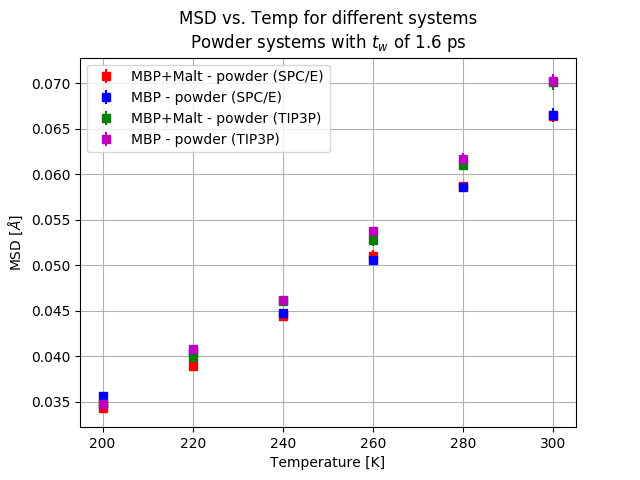
\includegraphics[width=0.7\textwidth]{./MSD/tempS-powders-tw2.png}
    
    \vspace{0.8cm}

    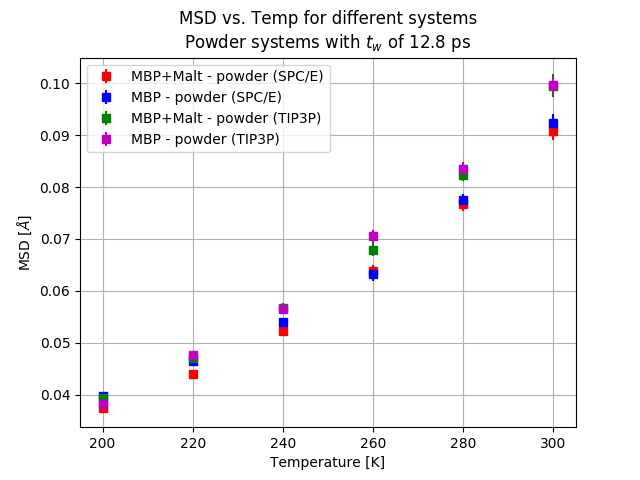
\includegraphics[width=0.7\textwidth]{./MSD/tempS-powders-tw13.png}

    \vspace{0.8cm}

    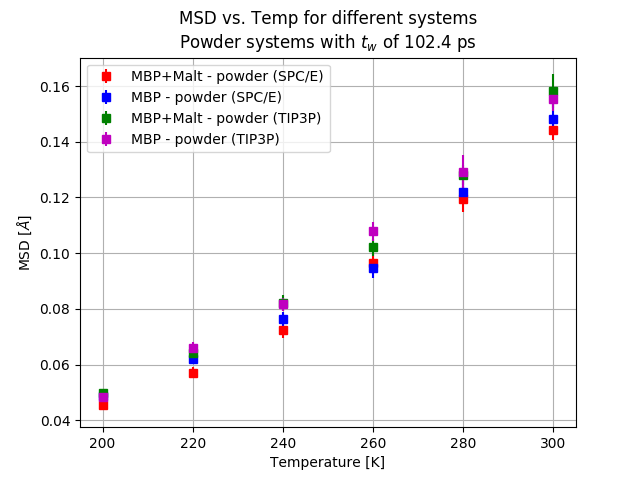
\includegraphics[width=0.7\textwidth]{./MSD/tempS-powders-tw102.png}
\end{figure}

\newpage

\begin{figure}[H]
\centering	
    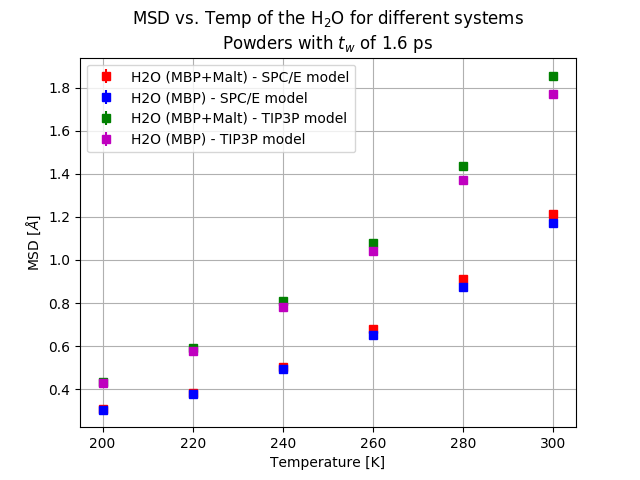
\includegraphics[width=0.7\textwidth]{./MSD/tempS-hpow-tw2.png}
    
    \vspace{0.8cm}

    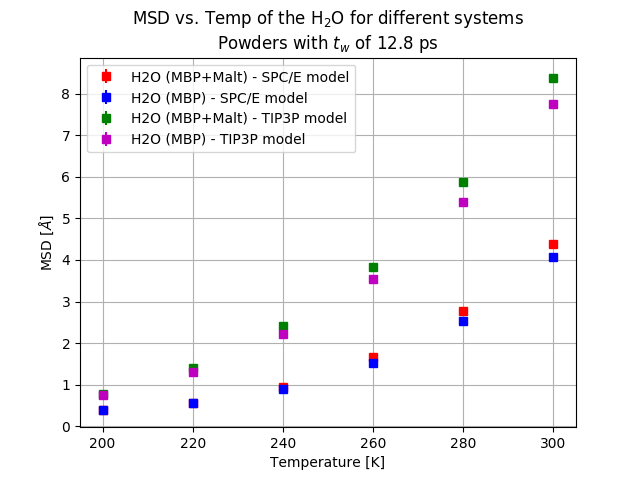
\includegraphics[width=0.7\textwidth]{./MSD/tempS-hpow-tw13.png}

    \vspace{0.8cm}

    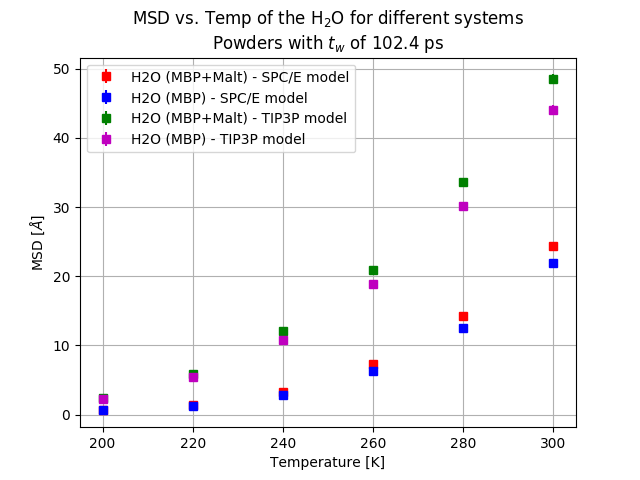
\includegraphics[width=0.7\textwidth]{./MSD/tempS-hpow-tw102.png}
\end{figure}

\begin{figure}[H]
\centering	
    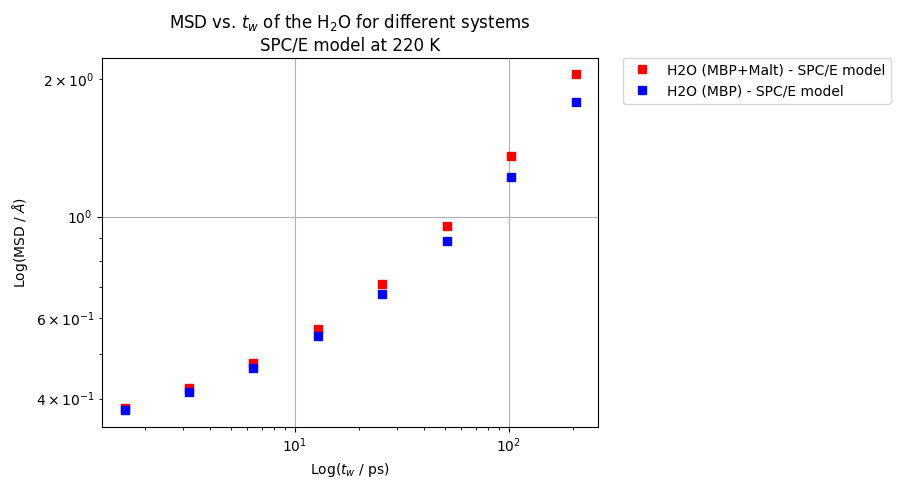
\includegraphics[width=0.65\textwidth]{./MSD/twS-hspce-ll220.png}
    
    \vspace{0.8cm}

    \includegraphics[width=0.65\textwidth]{./MSD/tws-spce-ll220.png}

    \vspace{0.8cm}

    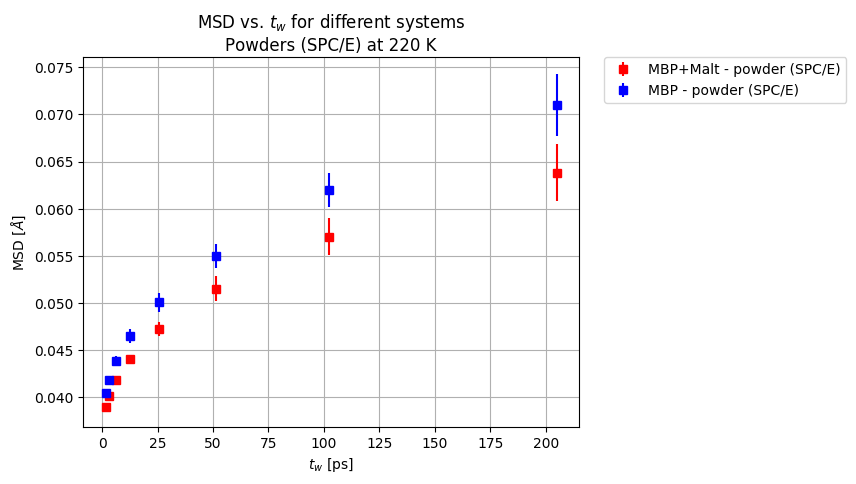
\includegraphics[width=0.625\textwidth]{./MSD/twS-spce220.png}
\end{figure}

\begin{figure}[H]
\centering	
    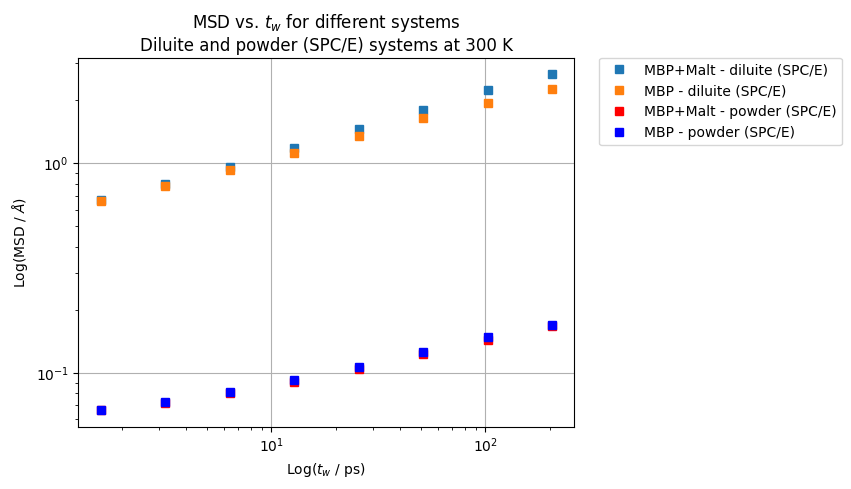
\includegraphics[width=\textwidth]{./MSD/twS-dil-spce-loglog300.png}
    
    \vspace{0.8cm}

    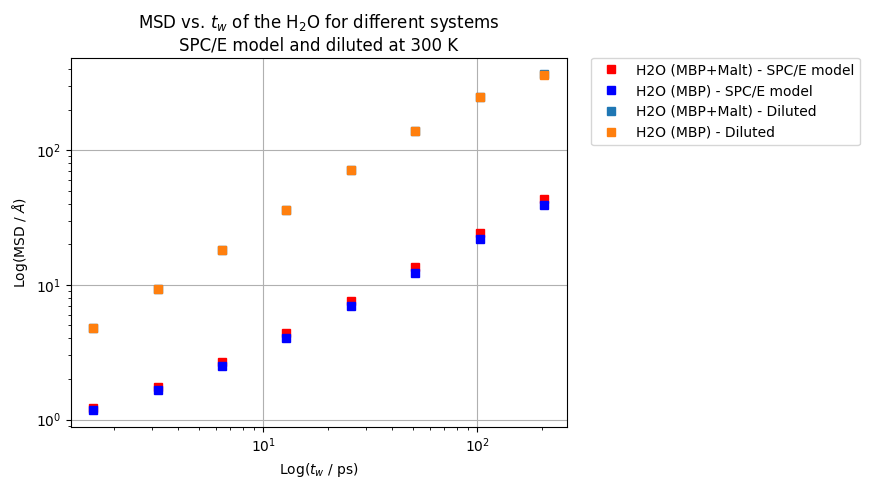
\includegraphics[width=\textwidth]{./MSD/twS-hspce-dil-ll300.png}
\end{figure}

%\begin{figure}[h] \centering
%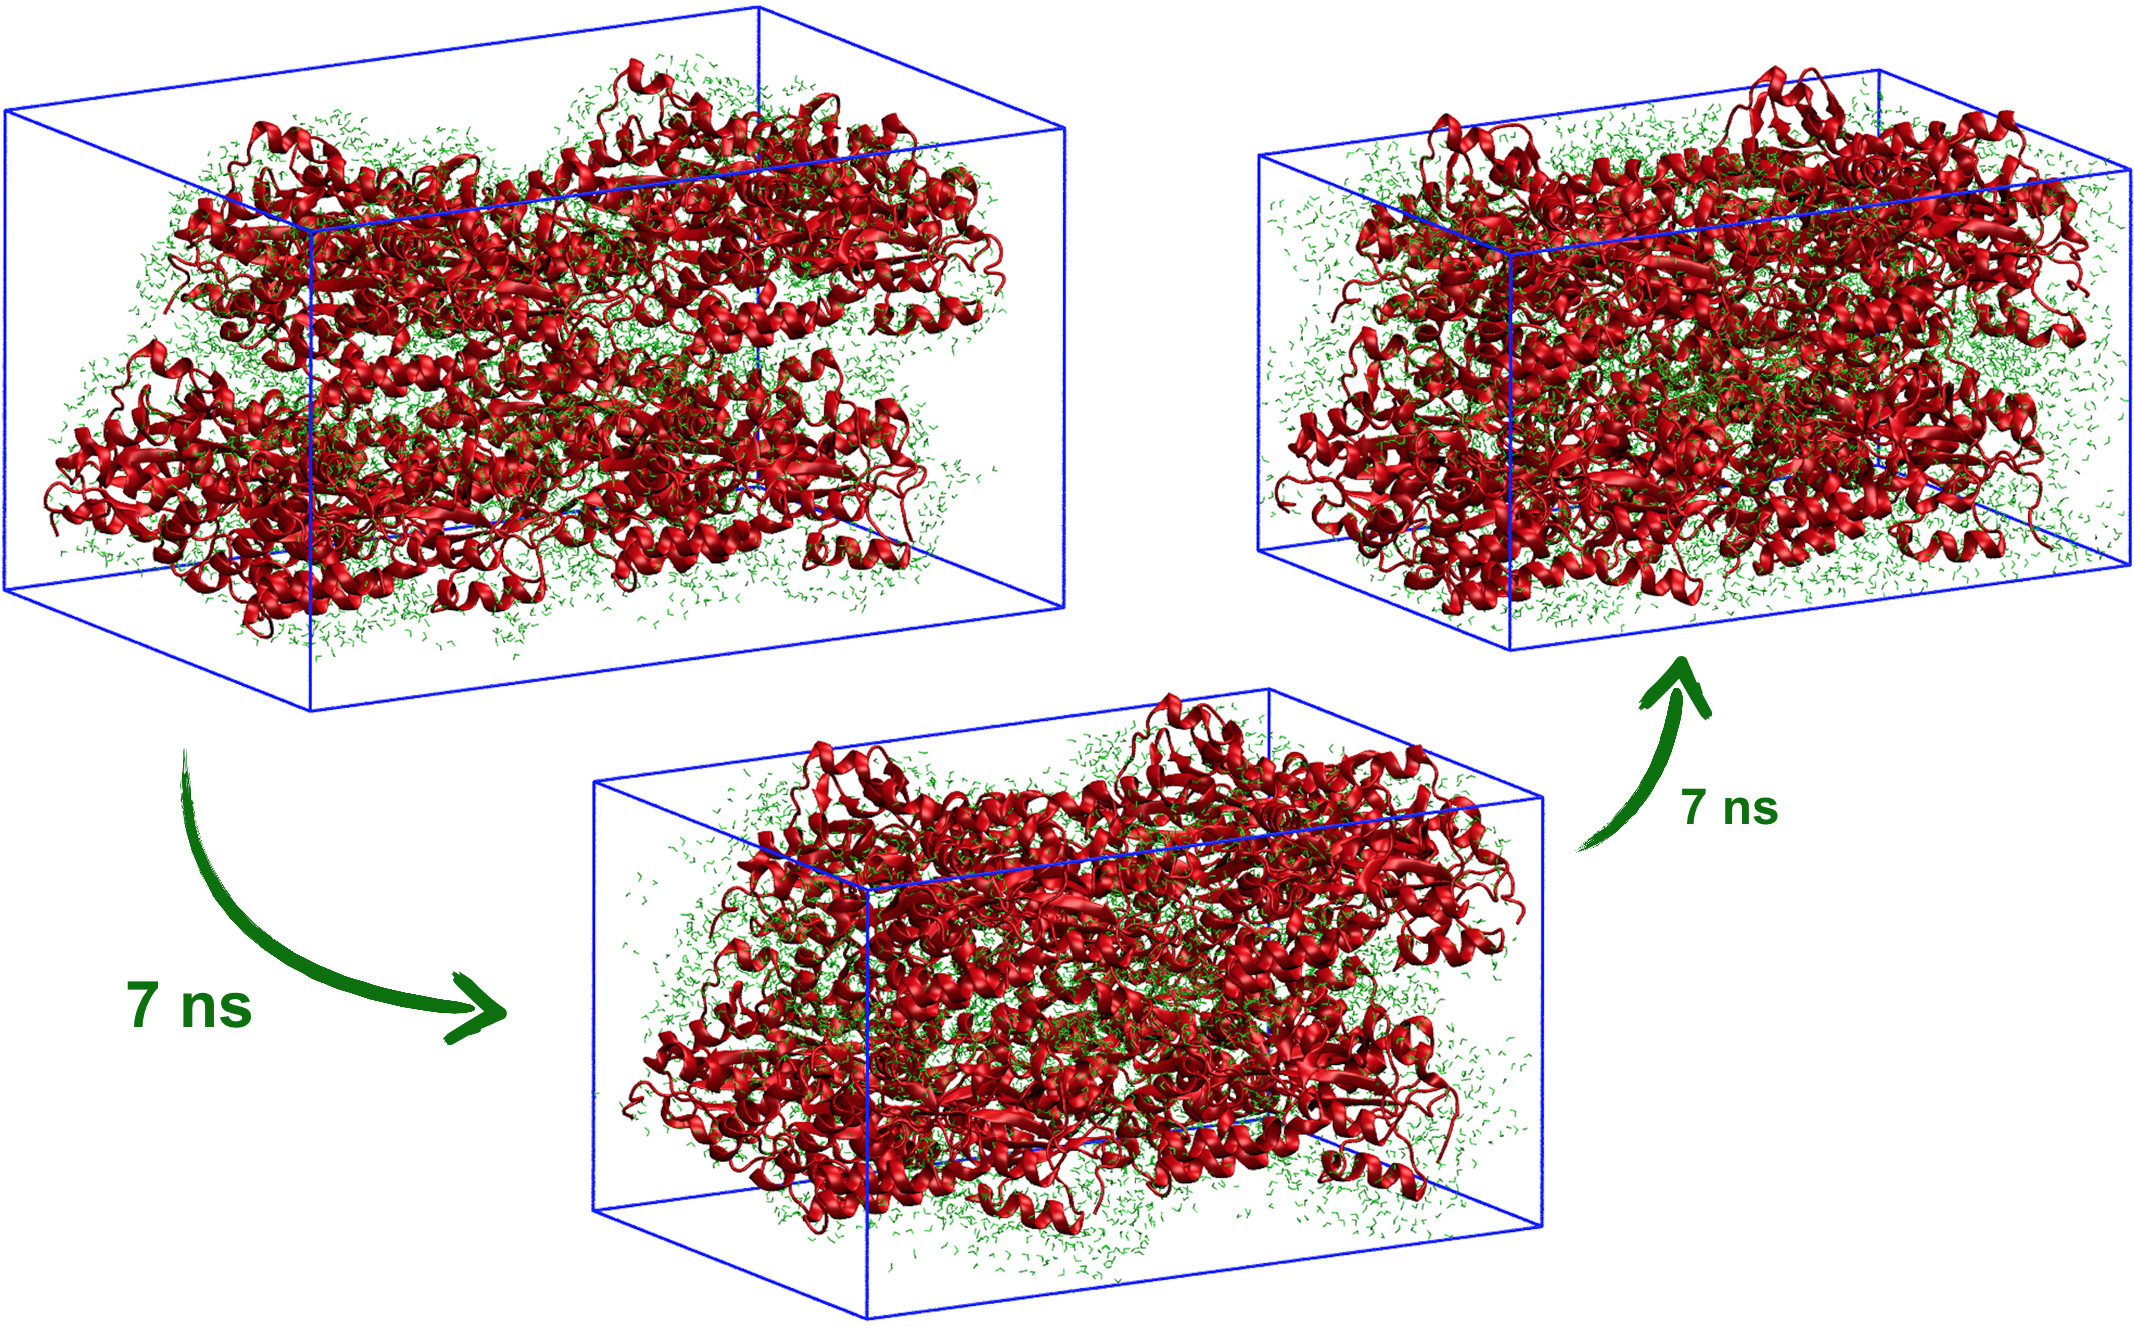
\includegraphics[width=0.9\textwidth]{./images/h1.jpg}\\
%\textbf{Tilt view}
%
%\vspace{0.8cm}
%
%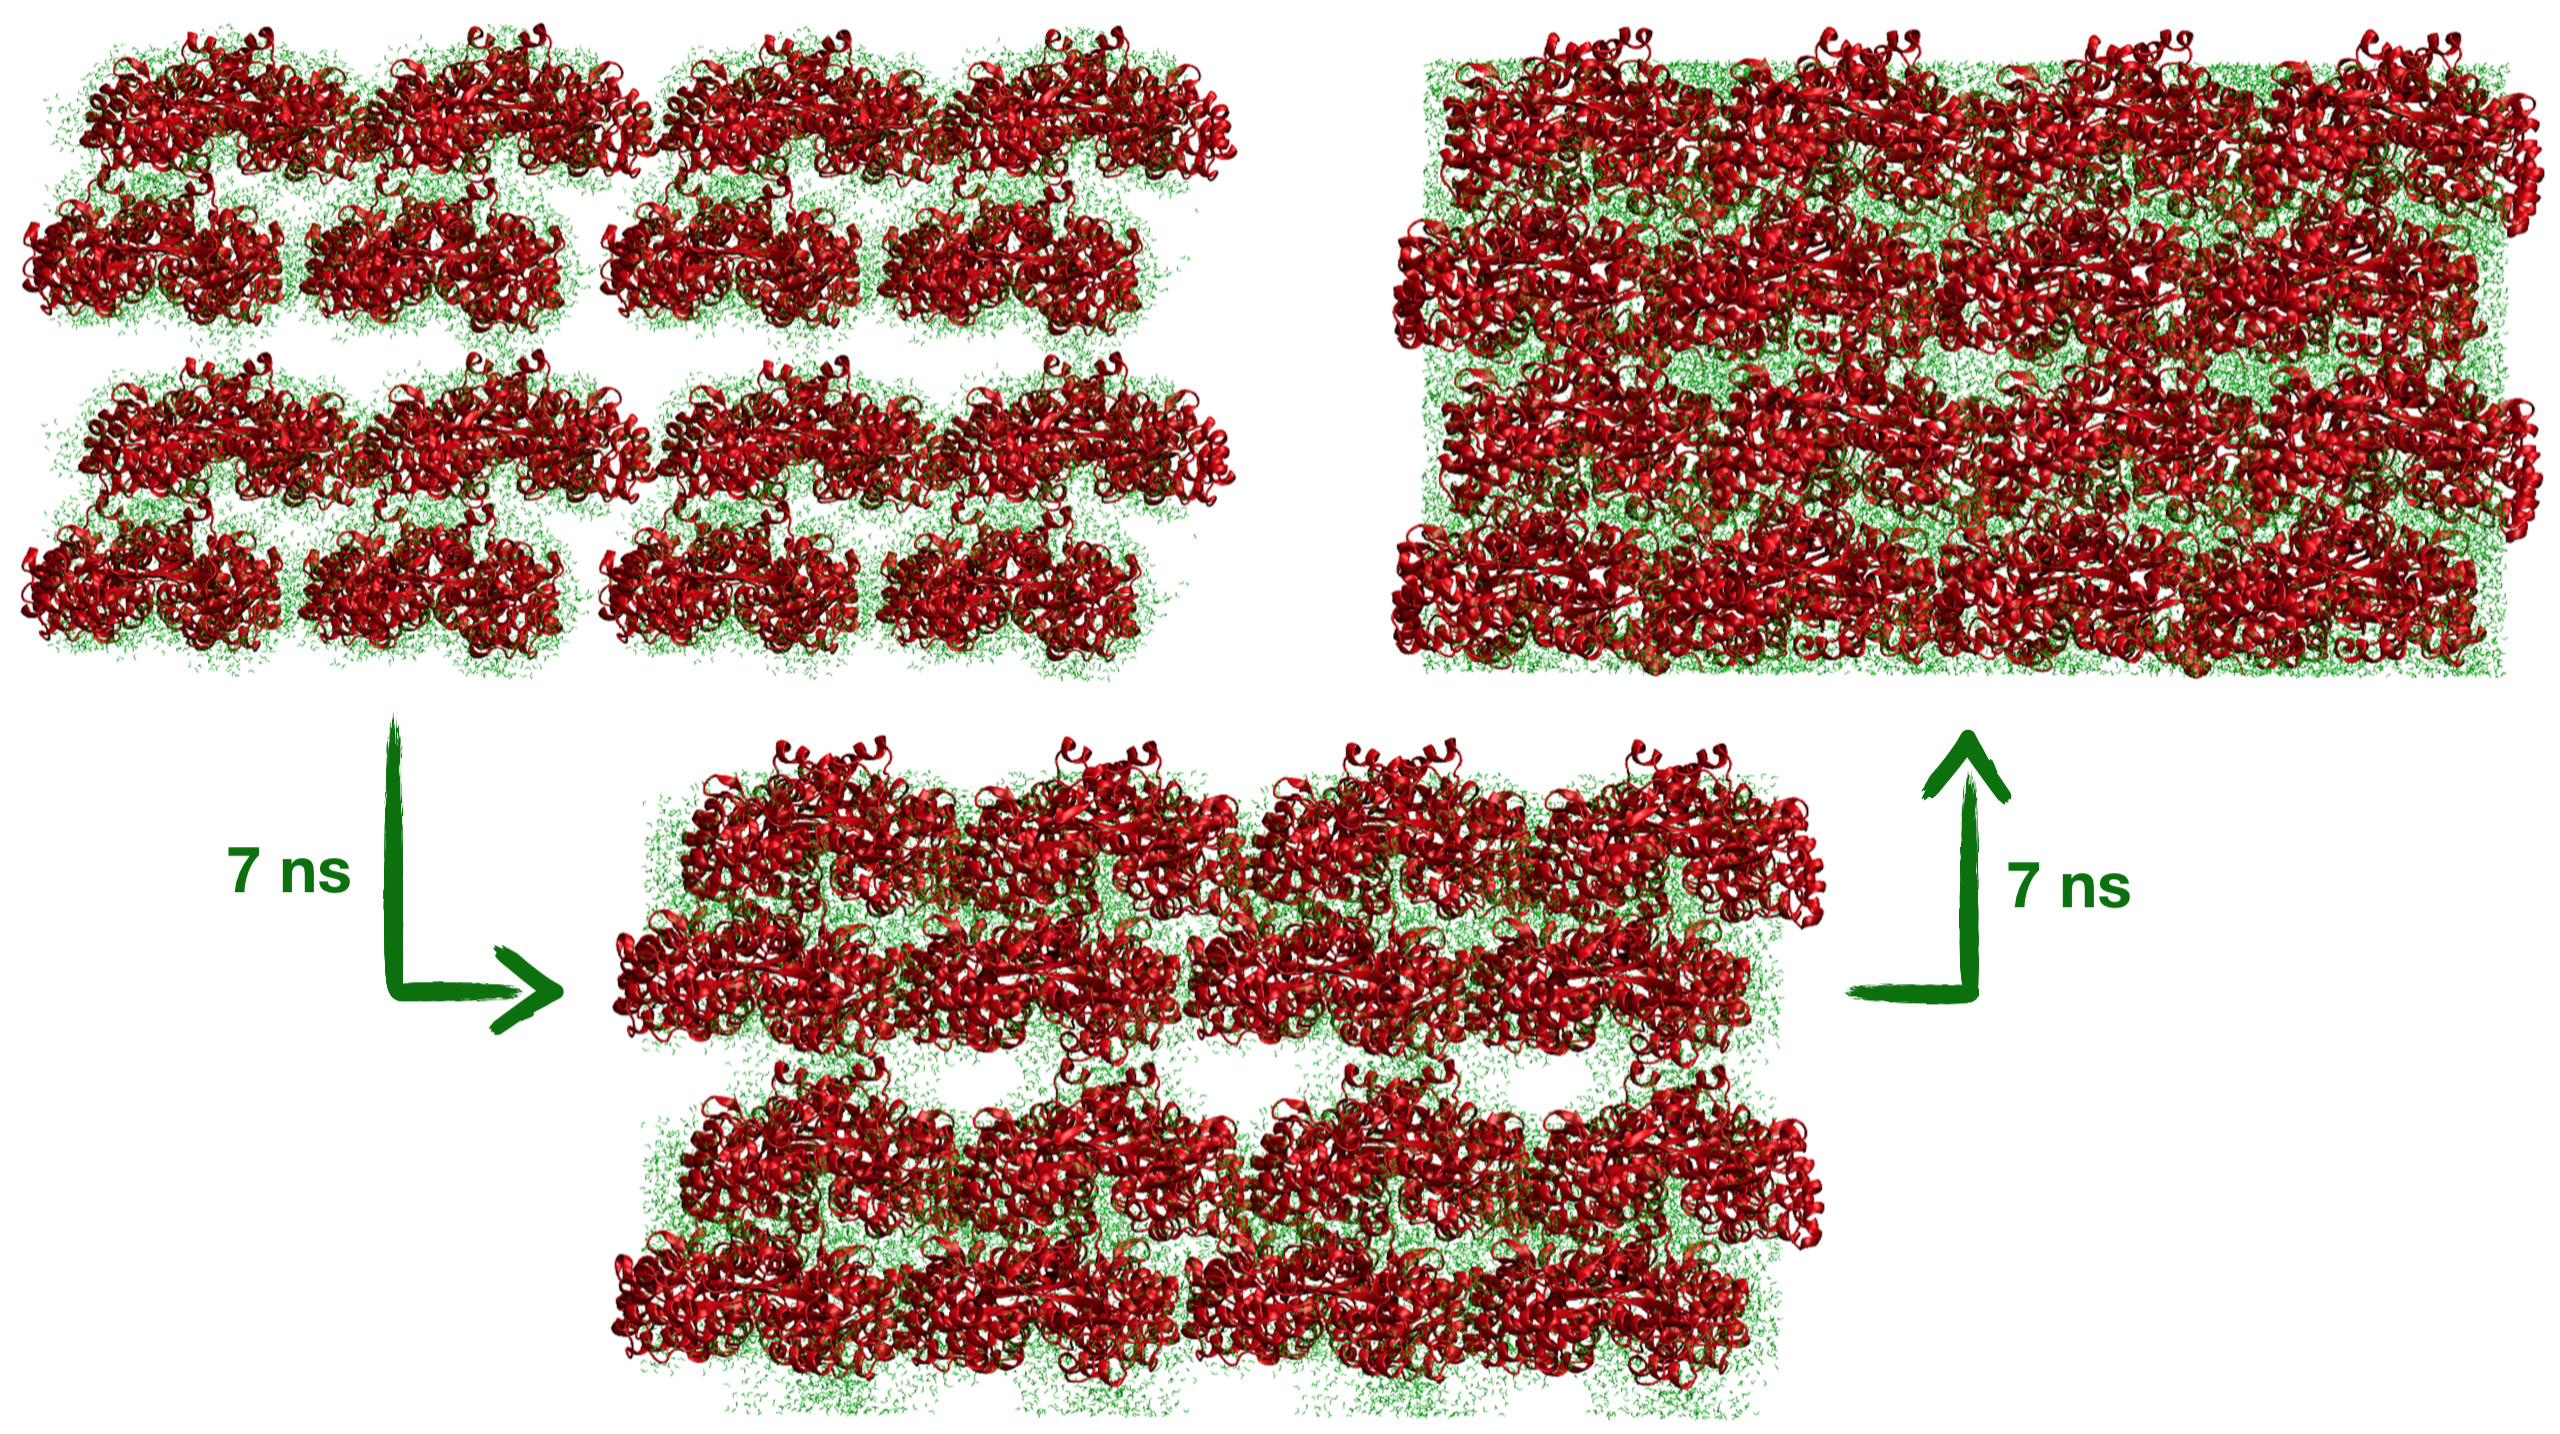
\includegraphics[width=\textwidth]{./images/h2.jpg}\\
%\textbf{Front view}\\
%\textit{{\small (here, the simulation box is replicated using two periodic images)}}
%\end{figure}


